\documentclass{standalone}

\usepackage{pgfplots,tikz,amsmath}
\begin{document}
        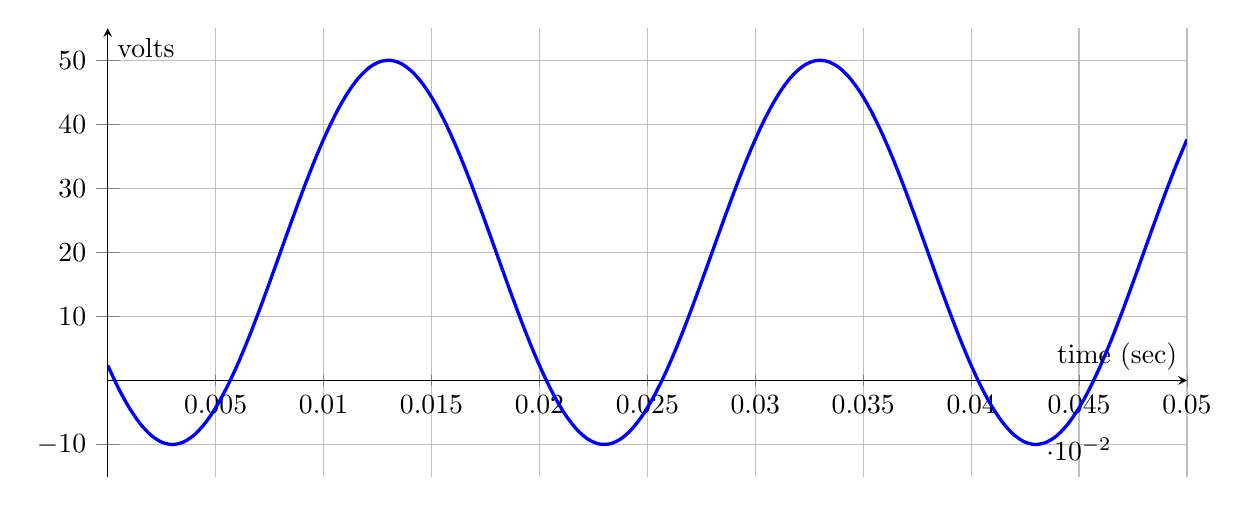
\begin{tikzpicture}
            \begin{axis}[axis lines=center, xmin=0, xmax=0.05, ymin=-15, ymax=55, grid,
                    domain=0:0.05, xlabel={time (sec)}, ylabel={volts},
                    xtick={0.005,0.01,0.015,0.02,0.025,0.03,0.035,0.04,0.045,0.05},
                    xticklabels={0.005,0.01,0.015,0.02,0.025,0.03,0.035,0.04,0.045,0.05},
                ytick={-10,10,20,30,40,50}, xscale=2]
                \addplot[smooth, very thick, blue, samples=100]
                {30*sin(deg(2*pi/0.02*(x-0.008)))+20};
            \end{axis}
        \end{tikzpicture}
\end{document}
